\documentclass[10pt,a4paper]{article}
\usepackage[margin=1.6cm]{geometry}
\usepackage[T1]{fontenc}
\usepackage{lmodern,booktabs,array,xcolor,amsmath,amssymb,hyperref,fancyhdr,microtype,graphicx,float}
\usepackage{pgfplots}
\pgfplotsset{compat=1.18}
\definecolor{navy}{HTML}{17365D}
\definecolor{blue}{HTML}{1F77B4}
\definecolor{orange}{HTML}{D95F02}
\definecolor{green}{HTML}{1B9E77}
\definecolor{purple}{HTML}{7570B3}
\hypersetup{colorlinks=true,linkcolor=navy,urlcolor=navy}
\pagestyle{fancy}\fancyhf{}\lhead{Controlled error geometry on GBnetwork}\rhead{7 September 2026}\cfoot{\thepage}
\setlength{\parindent}{0pt}\setlength{\parskip}{0.45em}
\newcommand{\PB}{\mathrm{PB}}
\newcommand{\Vm}{\lvert V\rvert}
\begin{document}

\begin{center}
{\LARGE\bfseries\color{navy} Controlled Error-Geometry Experiment on GBnetwork}\\[.25em]
{\small Fixed-norm directional intervention across PIGNN-GC, GridSFM, GridFM-GraphKit, and LUMINA}
\end{center}

\section{Question and conclusion}

The question is whether reconstructed AC power-balance inconsistency is more
sensitive to the direction of voltage-magnitude error outside a
training-derived solution subspace than to error within it.  The experiment
holds the error norm fixed separately for every held-out scenario, retains the
model's calibrated phase angle, and changes only the magnitude-error direction.

All four 40-epoch surrogate families exhibit the same directional contrast:
removing the off-subspace component reduces mean power balance (PB), whereas
removing the in-subspace component increases it.  The effect is largest for
PIGNN-GC and GridSFM, intermediate for GraphKit, and small but statistically
nonzero for LUMINA.  This is a diagnostic counterfactual that uses the Newton
reference state; it is \emph{not} a deployable correction.  The separate CSP
rows below are the practical frozen-output intervention.

\section{Frozen protocol}

GBnetwork Backbone v2 contains 37,022 converged 2224-bus AC power-flow
scenarios.  The split is \texttt{random\_split} with seed 42: 12,339 train,
12,339 validation, and 12,344 test scenarios.  The four inputs are the
best-validation checkpoints from the matched 40-epoch campaign.  Per-bus
magnitude offsets and circular angle offsets are fitted on training predictions
only and frozen before validation or test scoring.

For predicted and reference calibrated magnitudes, let
\[
 e=\hat v^C-v^\star,\qquad e^\parallel=P_ke,\qquad e^\perp=(I-P_k)e,
\]
where $P_k$ is fitted only to centered training reference magnitudes.  At each
test scenario and $\alpha\in\{0,.25,.5,.75,1\}$, the two counterfactuals are
\[
 \tilde e_\perp(\alpha)=\lVert e\rVert_2
 \frac{e^\parallel+\alpha e^\perp}{\lVert e^\parallel+\alpha e^\perp\rVert_2},\qquad
 \tilde e_\parallel(\alpha)=\lVert e\rVert_2
 \frac{\alpha e^\parallel+e^\perp}{\lVert\alpha e^\parallel+e^\perp\rVert_2}.
\]
No clipping or epsilon approximation was used; a zero original error maps to a
zero counterfactual, and a nonzero error with a zero denominator would fail the
run.  The scorer recomputes complex128 AC residuals from the modified complex
voltage.  Its GENCO-compatible per-bus score is
\[
 r_i^{\PB}=\begin{cases}
 \sqrt{\Delta P_i^2+\Delta Q_i^2},&i\in\mathrm{PQ},\\
 |\Delta P_i|,&i\in\mathrm{PV},\\0,&i\in\mathrm{slack},\end{cases}
 \qquad \mathrm{Mean\ PB}=\frac{1}{SN}\sum_{s,i}r_{is}^{\PB}.
\]

\subsection*{Validation-only rank selection}

Candidate ranks were $\{4,8,16,32,64\}$.  A rank was admissible only if CSP
did not worsen validation $\Vm$ RMSE for \emph{any} model.  Among admissible
ranks, the pre-declared objective minimized the mean of the four normalized
PB values $q_m(k)=\mathrm{PB}^{\mathrm{CSP}}_m(k)/\mathrm{PB}^{C}_m$.
Every candidate met the RMSE guardrail; $k^\star=16$ was selected before the
test split was scored.

\begin{center}\small
\begin{tabular}{lrrrrr}
\toprule
Rank $k$ & 4 & 8 & \textbf{16} & 32 & 64\\
\midrule
Mean $q_m(k)$ over four models & .272423 & .272030 & \textbf{.270474} & .271460 & .271975\\
\bottomrule
\end{tabular}
\end{center}

\section{Test results at frozen $k^\star=16$}

Table~\ref{tab:practical} distinguishes the calibrated model state from its
practical calibrated solution-subspace projection (CSP).  CSP improves both
the magnitude RMSE and Mean PB for all four families; the magnitude of this
practical gain is architecture dependent.

\begin{table}[H]
\centering\small
\caption{Frozen-output intervention on the 12,344-scenario test split.  C is
train-only calibration; CSP is C followed by $P_{16}$.}\label{tab:practical}
\begin{tabular}{lrrrr}
\toprule
Model & Mean PB (C) & Mean PB (CSP) & $\Vm$ RMSE (C) & $\Vm$ RMSE (CSP)\\
\midrule
PIGNN-GC & .14376 & .05690 & .01422 & .01289\\
GridSFM & .08660 & .05009 & .01179 & .00857\\
GridFM-GraphKit & 1.45564 & .07801 & .02090 & .02026\\
LUMINA & 1.83683 & .10291 & .02331 & .02326\\
\bottomrule
\end{tabular}
\end{table}

Figure~\ref{fig:direction} is the controlled mechanism experiment.  Every
curve is normalized by that model's calibrated Mean PB at $\alpha=1$; hence
all curves start at one and do not compare raw model quality.  Off-subspace
suppression reduces PB monotonically for PIGNN-GC and GridSFM.  It also reduces
PB for GraphKit and LUMINA, but only modestly.  The in-subspace control moves
in the opposite direction for every model.

\begin{figure}[h]
\centering
\begin{minipage}{.49\linewidth}\centering
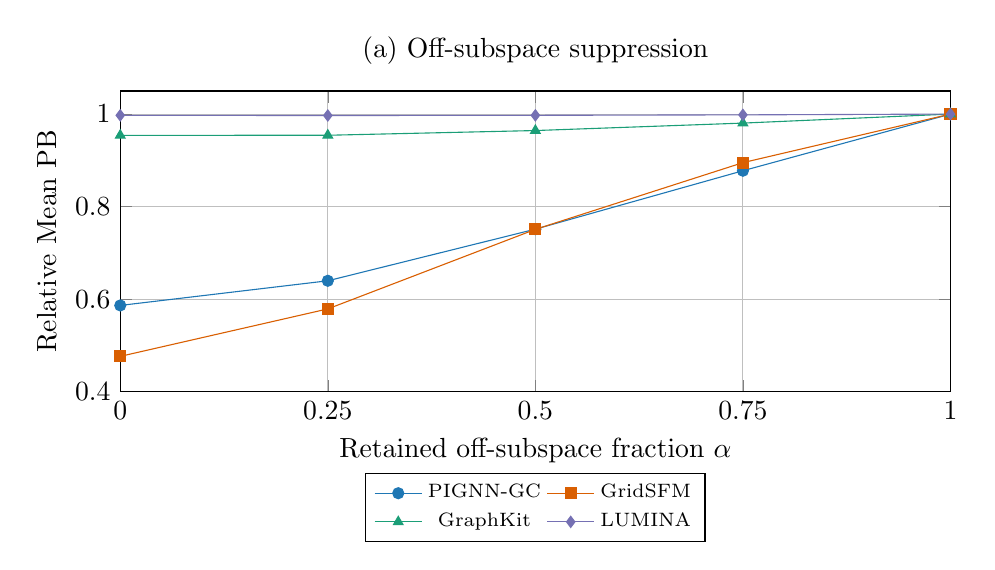
\begin{tikzpicture}
\begin{axis}[width=\linewidth,height=5.4cm, xlabel={Retained off-subspace fraction $\alpha$}, ylabel={Relative Mean PB},
title={(a) Off-subspace suppression}, xmin=0,xmax=1,ymin=.4,ymax=1.05,
xtick={0,.25,.5,.75,1},grid=major,legend style={font=\scriptsize,at={(.5,-.27)},anchor=north,legend columns=2}]
\addplot[color=blue,mark=*] coordinates {(0,.5863)(.25,.6396)(.5,.7512)(.75,.8775)(1,1)};\addlegendentry{PIGNN-GC}
\addplot[color=orange,mark=square*] coordinates {(0,.4762)(.25,.5788)(.5,.7508)(.75,.8950)(1,1)};\addlegendentry{GridSFM}
\addplot[color=green,mark=triangle*] coordinates {(0,.9540)(.25,.9542)(.5,.9644)(.75,.9805)(1,1)};\addlegendentry{GraphKit}
\addplot[color=purple,mark=diamond*] coordinates {(0,.9973)(.25,.9969)(.5,.9973)(.75,.9983)(1,1)};\addlegendentry{LUMINA}
\end{axis}\end{tikzpicture}
\end{minipage}\hfill
\begin{minipage}{.49\linewidth}\centering
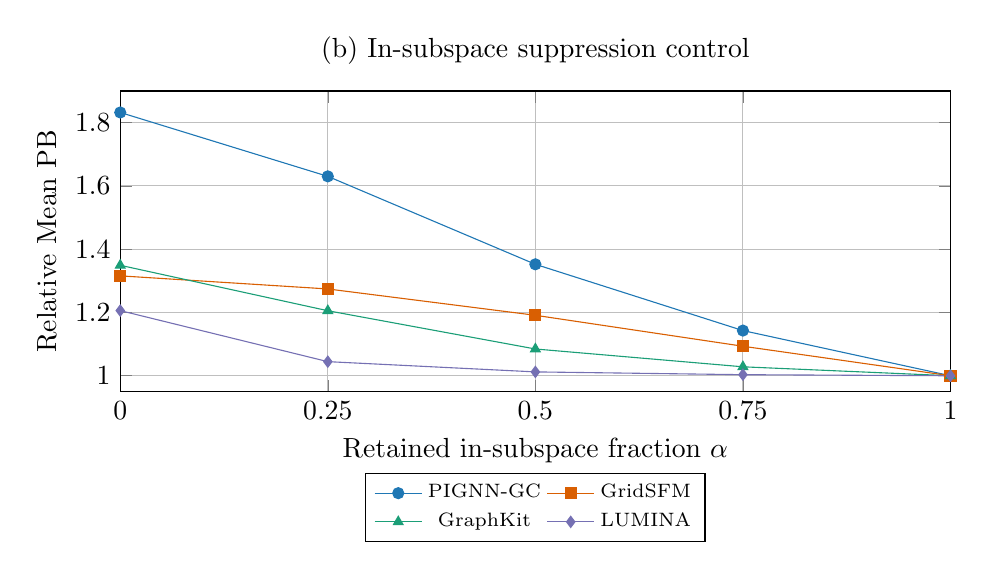
\begin{tikzpicture}
\begin{axis}[width=\linewidth,height=5.4cm, xlabel={Retained in-subspace fraction $\alpha$}, ylabel={Relative Mean PB},
title={(b) In-subspace suppression control}, xmin=0,xmax=1,ymin=.95,ymax=1.9,
xtick={0,.25,.5,.75,1},grid=major,legend style={font=\scriptsize,at={(.5,-.27)},anchor=north,legend columns=2}]
\addplot[color=blue,mark=*] coordinates {(0,1.8320)(.25,1.6301)(.5,1.3522)(.75,1.1428)(1,1)};\addlegendentry{PIGNN-GC}
\addplot[color=orange,mark=square*] coordinates {(0,1.3157)(.25,1.2743)(.5,1.1911)(.75,1.0933)(1,1)};\addlegendentry{GridSFM}
\addplot[color=green,mark=triangle*] coordinates {(0,1.3491)(.25,1.2055)(.5,1.0846)(.75,1.0283)(1,1)};\addlegendentry{GraphKit}
\addplot[color=purple,mark=diamond*] coordinates {(0,1.2059)(.25,1.0446)(.5,1.0122)(.75,1.0034)(1,1)};\addlegendentry{LUMINA}
\end{axis}\end{tikzpicture}
\end{minipage}
\caption{Fixed-norm directional diagnostic at $k^\star=16$.  Each point changes
only the orientation of the calibrated magnitude error and retains the
calibrated phase angle.  Lower is better.}\label{fig:direction}
\end{figure}

\begin{table}[H]
\centering\footnotesize
\caption{Endpoint robustness at $\alpha=0$.  $\Delta\PB$ is relative to
$\alpha=1$; CIs are 95\% paired bootstrap intervals over 12,344 scenarios.}\label{tab:endpoint}
\begin{tabular}{lrrr}
\toprule
Model & Off $\Delta\PB$ [95\% CI] & PB lower (off) & In-control $\Delta\PB$ [95\% CI]\\
\midrule
PIGNN-GC & $-.05947$ [$-.05991,-.05904$] & 100.000\% & $+.11962$ [$+.11806,+.12118$]\\
GridSFM & $-.04536$ [$-.04569,-.04507$] & 100.000\% & $+.02734$ [$+.02706,+.02763$]\\
GraphKit & $-.06690$ [$-.06715,-.06665$] & 99.992\% & $+.50814$ [$+.50227,+.51417$]\\
LUMINA & $-.00497$ [$-.00503,-.00490$] & 99.174\% & $+.37820$ [$+.37265,+.38403$]\\
\bottomrule
\end{tabular}
\end{table}

\section{Interpretation and limitations}

The experiment supports a directional explanation beyond total voltage-error
magnitude: rotating the same error norm away from $e^\perp$ is associated with
lower AC PB, while suppressing $e^\parallel$ is harmful.  It does not identify
the empirical SVD subspace with the AC-feasible set, does not prove that every
off-subspace direction is physically invalid, and does not establish a causal
architecture ranking.  GraphKit and LUMINA show a much weaker off-subspace
effect than PIGNN-GC and GridSFM; this heterogeneity should be retained in any
paper figure or claim.  The subspace is fitted to the training operating
distribution, so this report does not establish out-of-distribution transfer.

\section{Reproducibility record}

The Stage-1 validation JSONs, frozen rank decision, Stage-2 summaries, and
per-scenario PB arrays are saved under
\texttt{results/controlled\_geometry\_20260905/}.  Stage 2 used the frozen
common rank only after the validation decision was recorded.  The largest
absolute fixed-norm error was $8.88\times10^{-16}$, the largest $\alpha=1$ PB
reproduction error was exactly zero, and no zero-denominator or invalid case
occurred.  These checks rule out clipping, norm drift, or a mismatch between
the counterfactual's $\alpha=1$ endpoint and the calibrated prediction.

\end{document}
